\documentclass[14pt]{report}
\usepackage{graphicx}
\usepackage{longtable}
\usepackage{rotating}
\usepackage[acronym,toc]{glossaries}
\usepackage{biblatex}
\renewcommand{\rmdefault}{ptm}
\usepackage[utf8]{inputenc}
\usepackage{mathptmx}
\usepackage{multirow}
\usepackage{amsmath}
\usepackage[table,xcdraw]{xcolor}
\usepackage{setspace}
\usepackage[]{siunitx}
\usepackage[top=1in, bottom=1in, left=1in, right=1in]{geometry}

\makenoidxglossaries

\newacronym{mcu}{MCU}{Micro-Controller-Unit}

\addbibresource{References.bib}

\begin{document}

\begin{titlepage}
\begin{center}
\begin{Large}
\textbf{A Project Report \\ on} \\[0.1in]
\end{Large}
\begin{LARGE}
\begin{singlespace}
\textbf{\uppercase{Compact Short Range Frequency Modulated Continuous Wave Radar for Enhanced Vision in Unmanned Ground Vehicle}}
\end{singlespace}
\end{LARGE}
\end{center}
\begin{center}
\begin{Large}
\it{Submitted in the Partial Fulfillment of the Requirements \\
for the award of} \\[0.2in]
\end{Large}
\begin{LARGE}
\textbf{Bachelor of Technology \\ in \\[0.1in] Electronics \& Communication Engineering}
\end{LARGE} \\[0.2in]
By\\[0.05in]
\begin{large}
\textbf{Subha Sarkar} \\
(20145120) \\
\textbf{Tushar Kumar} \\
(20145073) \\
\textbf{Ashish Kumar Jha} \\
(20145002) \\[0.1in]
\end{large}
Under the guidance of \\[0.05in] 
\begin{large}
\textbf{Dr. Yogendra Kumar Prajapati} \\[0.05in]
\textbf{Assistant Professor} \\[0.25in]
\end{large}
\end{center}
\begin{center}

\includegraphics[scale=0.05]{MNNIT.png} \\[0.25in]
\begin{center}
\begin{Large}
\textbf{Department of Electronics \& Communication Engineering \\
Motilal Nehru National Institute of Technology Allahabad \\
Allahabad - INDIA \\ [0.05in]} 
(January , 2018)
\end{Large}
\end{center}
\end{center}
\end{titlepage}
\newpage
\pagenumbering{roman}

\begin{center}
\section*{UNDERTAKING}
\addcontentsline{toc}{section}{Undertaking}
\end{center}
\begin{Large}
\begin{onehalfspace}
We declare that the work presented in this project titled \textbf{Compact Short Range Frequency Modulated Continuous Wave Radar for Enhanced Vision in Unmanned Ground Vehicle} submitted to the Department of Electronics and Communication Engineering, Motilal Nehru National Institute of Technology Allahabad for the award of the \textbf{Bachelor of Technology} degree in Electronics and \& Communication Engineering is our original work. We have not plagiarized or submitted the same work for the award of any other degree. In case this undertaking is found incorrect, we accept that our degree may be unconditionally withdrawn.
\end{onehalfspace}
\end{Large}

\begin{Large}
\begin{onehalfspace}
\begin{flushleft}
\today \\
Allahabad , INDIA
\end{flushleft}
\end{onehalfspace}
\end{Large}

\begin{Large}
\begin{onehalfspace}
\begin{flushright}
Subha Sarkar \\[0.2in]
Tushar Kumar \\[0.2in]
Ashish Kumar Jha \\[0.1in]
\end{flushright}
\end{onehalfspace}
\end{Large}
\newpage

\begin{center}
\begin{LARGE}
\textbf{Department of Electronics \& Communication Engineering \\
Motilal Nehru National Institute of Technology Allahabad \\
Allahabad - INDIA \\}
\end{LARGE}
\end{center}

\begin{center}
\section*{CERTIFICATE}
\addcontentsline{toc}{section}{Certificate}
\end{center}

\begin{Large}
\begin{onehalfspace}
This is to certify that the work contained in the project titled 
\textbf{Compact Short Range Frequency Modulated Continuous Wave Radar for Enhanced Vision in Unmanned Ground Vehicle},
submitted by \textbf{Subha Sarkar}, \textbf{Tushar Kumar} and \textbf{Ashish Kumar Jha} in the partial fulfillment of the
requirement for the award of Bachelor of Technology in Electronics \& Communication
Engineering to the Electronics \& Communication Engineering Department, Motilal
Nehru National Institute of Technology, Allahabad, is a bonafide work of the students
carried out under my supervision.
\end{onehalfspace}
\end{Large}

\begin{Large}
\begin{onehalfspace}
\begin{flushleft}
\today \\
Allahabad , INDIA
\end{flushleft}
\end{onehalfspace}
\end{Large}

\begin{Large}
\begin{onehalfspace}
\begin{flushright}
(Yogendra Kumar Prajapati) \\
Assistant Professor \\
ECE Department \\
MNNIT Allahabad \\[0.1in]
\end{flushright}
\end{onehalfspace}
\end{Large}
\newpage

\begin{center}
\section*{ACKNOWLEDGEMENT}
\addcontentsline{toc}{section}{Acknowledgement}
\end{center}
\begin{Large}
\begin{onehalfspace}
The successful completion of this project required a lot of guidance and assistance from many people and we find ourselves extremely privileged to have got this all along the completion of the project. All that we have done is only due to such supervision and assistance and we thank them all whole heartedly.

We respect and thank \textbf{Dr. Yogendra Kumar Prajapati}, for providing us an opportunity to do the project work in MNNIT Allahabad and giving us all support and guidance which helped us complete the project within the alloted time. We are extremely thankful to him for providing such a nice support and guidance, although he had busy schedule managing his own duties.

We owe our heartiest gratitude to \textbf{Dr. Vijaya Bhadauria} \textit{(Head of the department)}, who took keen interest on our project work and guided us all along, till the completion of our project work by providing all the necessary information for developing a good system.

We are thankful to and fortunate enough to get constant encouragement, support and guidance from all Teaching staffs of Department of Electronics \& Communication Engineering , MNNIT Allahabad which helped us in successfully completing our project work. Also, We would like to extend our sincere gratitude to all staff in laboratory for their timely support.

\end{onehalfspace}
\end{Large}

\begin{Large}
\begin{onehalfspace}
\begin{flushleft}
\today \\
Allahabad , INDIA
\end{flushleft}
\end{onehalfspace}
\end{Large}

\begin{Large}
\begin{onehalfspace}
\begin{flushright}
Subha Sarkar \\[0.2in]
Tushar Kumar \\[0.2in]
Ashish Kumar Jha \\[0.1in]
\end{flushright}
\end{onehalfspace}
\end{Large}
\newpage

\begin{center}
\section*{ABSTRACT}
\addcontentsline{toc}{section}{Abstract}
\end{center}
\begin{Large}
\begin{onehalfspace}
A microwave RAdio Detection And Ranging sensor can detect targets through fog, smoke and some other solid objects. It is unlike camera, ultrasonic, LIght Detection And Ranging where these are limited to visual targets only. This makes microwave radar sensor very useful in applications like reconnaissance, search and rescue, Hazardous environment exploration, mapping, navigation and automotive. Most of the components are found in small footprints which can be easily mounted on a custom Print Circuit Board for size reduction.
 
\hspace{0.5in} To detect range a simple un-modulated Doppler radar carrier is frequency modulated to produce a chirp signal using VCO and a function generator. The time difference corresponds to frequency difference obtained through mixer. Multiple objects means more frequency components which can be obtained through FFT. It requires an RF/microwave transceiver circuit and an ADC front-end circuit to obtain the digital data for further digital processing. To increase the speed of mapping by manifold (which is crucial in tactical operations), an FPGA would be used to sample data from ADC, compute FFT \& provide the final frequency components to the application processor. An application processor would be used to implement algorithms for calculating ranges, identify targets from data available through other sensors, source and channel coding for transmission and GUI. A lot of the implementations have a rotating radar which construct a 2-D field in azimuth plane using accumulation of 1-D points. This decreases the speed of mapping in time sensitive surveillance operation. In this proposal we would experiment a high speed short range scanning radar using array of two or more radar sensors providing data to a computer (Application processor + FPGA). This would allow to localize object in azimuth plane with enhanced mapping speed. This has advantage of having a small hardware (means better portability), fast scanning rate and better reliability.
\end{onehalfspace}
\end{Large}
\newpage

\begin{large}
\addcontentsline{toc}{section}{Contents}
\tableofcontents{}

\newpage
\addcontentsline{toc}{section}{List of Figures}
\listoffigures{}

\newpage
\addcontentsline{toc}{section}{List of Tables}
\listoftables{}
\end{large}

\newpage
\printnoidxglossary[type=acronym,title={Abbreviations}]

\pagenumbering{arabic}

\begin{Large}
\chapter{INTRODUCTION}
Short Range Microwave radar \cite{strohm2005development} is a continuously growing field of research in field of robotics and automotive. These microwave radar are being actively used to develop highly reliable sensors for Advanced Driver Assistance System (ADAS) in Automotive industry. The signal used for finding ranges in radar systems is an electromagnetic (EM) wave at microwave frequencies. The main advantage of radar systems compared to other altenatives such as sonar and lidar is the immunity to weather conditions and potential for lower cost realization. It requires a directional radar, RF front-end, compact \& low-power DSP computer to implement the sensor \cite{charvatres}. 
\section{Motivation}
Adaptive cruise control, navigation, search and surveillance, high resolution imaging and mapping, space flight, and sounding are the current applications worldwide. There are other many sensors available like stereo-camera which can provide visual data. However for the application of aforesaid navigation and cruise control it would require a lot computation effort to determine the distance of objects in responsive amount of time. With visual data, some non-reliable algorithmic process has to be followed which gives visual depth with highest "probability" of accuracy. When deployed in practical environments, the visual data in highly unreliable. Alternatively a LiDAR sensor can be used but it may not work during fog, mist etc. Another safety concern is the car’s ability to detect lightly-colored objects in real-time, such as nearby white vehicles.\\	
	A directional electromagnetic sensor is a better option which can not only provide distance of objects in front of it but also the angular position of the objects. In LiDAR, to detect angular position a single sensor has to be mechanically rotated. The mechanical rotation limits the speed at which it can sweep the area to detect targets, hence degrade agility of the vehicle. If a array of LiDAR sensor is used, it would take a lot of space and power. However the LiDAR sensor can be used to provide an additional safety layer. \\
	We want to develop our own design of such compact radar sensors with anticipated improvement in its angular resolution. In addition, it would allow to get  knowledge of Signal Analysers, Vector Network Analysers, FPGAs (for digital signal processing), High-frequency PCB designs etc.
\section{Present State of the Art}
Recently in 2017, industry leaders demonstrated recently developed small integrated sensors (AWR/IWR series from Texas Instruments Inc., Drive360 from Analog Devices Inc., MR2001 from NXP Semiconductors and more). All the principle components are integrated in a single silicon chip (in case of AWR) or in a single PCB presenting a very comfortable way for automotive engineers to test and deploy these sensors. However for more custom applications where modifications are required for better functionality it is required to analyse the present state of the art and modify/re-develop if required.
\section{Problem Statement}
Our project goal is development of compact frequency modulated continous wave radar for navigation and cruise control of unmanned ground vehicles. The design is done to improve the angular resolution of the system. The objectives are listed as following :
\begin{enumerate}
\item Simulating all possible modules in simulation software (CST or HFSS).
\item Development of individual modules in Print Circuit Board and thorough testing.
\item Integrating all the modules to form a complete PCB radar.
\item Demonstration.
\end{enumerate}
\section{Proposed Solution and Design Effort}
	The configuration of Radar would be Bistatic and it would use continous wave. As opposed to a continous wave radar, a pulse radar uses a complicated matched filter which requires not only complex electronic systems but also capital. We are making a bistatic radar to avoid duplexer. A duplexer is also a complicated device requiring great amount of isolation between ports. Any appreciable mismatch can cause damage to the sensor. Taking into account of modern microstrip antenna size, it is more safe and easy to make a bistatic radar than a monostatic radar. \\
	The frequency range of operation we have selected is S-band. At this range all the Integrated-Circuits are available at low cost. This is due to existance of ISM band (2.4 GHz) in S-band which covers wide variety products available in market. For compactness we would use microstrip antennas. It would be simulated using HFSS then fabricated in a PCB.
\section{Report Organisation}
\chapter{Basics of RADAR (RAdio Detection And Ranging)}
	The electromagnetic waves are reflected if they meet an electrically leading surface. If these reflected waves are received again at the place of their origin, then that means an obstacle is in the propagation direction. Electromagnetic energy travels through air at a constant speed, at approximately the speed of light. This energy normally travels through space in a straight line, and will vary only slightly because of atmospheric and weather conditions. By using of special radar antennas this energy can be focused into a desired direction. Thus the direction (in azimuth and elevation) of the reflecting objects can be measured. These principles can basically be implemented in a radar system, and allow the determination of the distance, the direction and the height of the reflecting object.
	
Radar units usually work with very high frequencies. Reasons for this are:
\begin{itemize}
\item quasi-optically propagation of these waves.
\item High resolution (the smaller the wavelength, the smaller the objects the radar is able to detect).
\item Higher the frequency, smaller the antenna size at the same gain.
\end{itemize}

\section{Advantages}
Radar has many advantages compared to an attempt of visual observation:
\begin{itemize}
\item Radar is able to operate day or night, in lightness or darkness over a long range;
\item Radar is able to operate in all weathers, in fog and rain, it can even penetrate walls or layers of snow;
\item Radar has very broad coverage; it is possible to observe the whole hemisphere;
\item Radar detects and tracks moving objects, a high resolution imaging is possible, that results in an object recognition;
\item Radar can operate unmanned, 24 hours a day, 7 days a week.
\end{itemize}

\section{Miniature FMCW Radar}

\begin{figure}
\centering
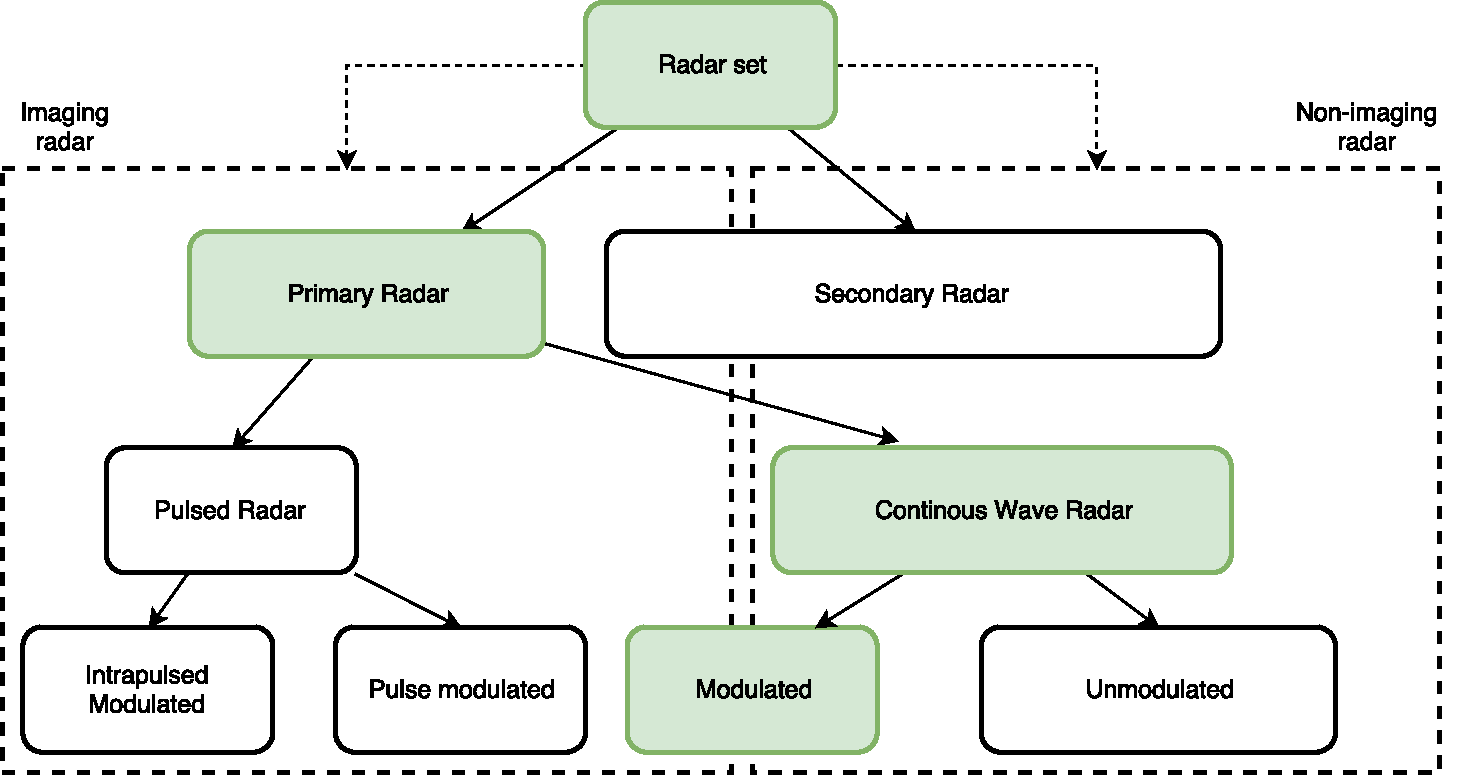
\includegraphics[width = 6in]{radar_classification.pdf}
\caption{Radar classification (The project belongs to the highlighted category)}
\end{figure}	

The configuration of radar is bistatic.
\section{Signal Processing}
		\subsection{Brief} The signal processing chain starts from the IF amplifier. An ADC samples the IF signal and send the data to the FPGA (DSP). The FPGA is the Cyclone V SoC from Intel (Altera). The FPGA performs the real time FFT to provide the frequency components.
		\subsection{Transmitter stage}
		The power amplifier is responsible for providing maximum power to the antenna. Unfortunately due to certain factors like antenna gain, impedance mismatch, and other losses which are related to antenna efficiency (conduction losses, dielectric losses).	
		The phase noise of the VCO should be as minimum as possible for better resolution. If not so then the phase noise tail would corrupt the wanted signal reflected back from the target.
		
\begin{figure}
\centering
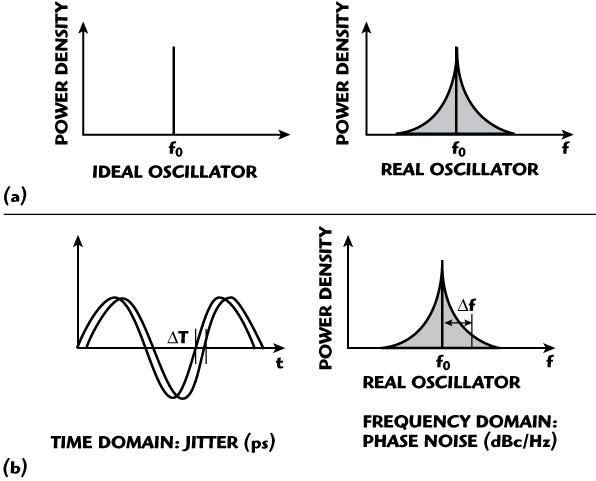
\includegraphics[width=4in]{Synergy_Microwave_Corporation_Jitter_and_Phase_Noise.jpg}
\caption{Phase noise and jitter}
Source : Synergy Microwave Corporation
\end{figure} 

		\subsection{Receiver stage}
		Typical received signal power is found to be around -150dBm to -30dBm. So these are needed to be amplified before being fed into mixer. A low noise amplifier is required for this purpose. 
		Phase noise is a key parameter for transceivers
		\subsection{IF amplifier stage}
		\subsection{Analog to Digital Converter}
		\subsection{FPGA-Digital Signal Processing}
\section{Component Research}
Components selected here are referenced from MIT Lincoln Laboratory project of FMCW radar \cite{charvatres}. However aforementioned source uses Mini-Circuits$^{\textregistered}$ off-the-shelf components for quick prototyping and allowing students to replicate the project for learning. We have learnt a lot from the meticulous documentation and have carefully selected components to suit them better with our design and allocated budget. 
Following are the part list and description :
\begin{enumerate}
\item \textbf{SMA} Connector  : As opposed to BNC connector SMA supports wider bandwidth from 0-18GHz. The inside tapered structure reduces the mismatch providing very low return loss.
\item \textbf{MAX2751} (VCO) -
\begin{itemize}
\item Output Power : -2dBm (After power on)
\item Phase noise : -92dBc @ 100KHz offset
\end{itemize}
\item \textbf{LT5512} (Mixer) :
\begin{itemize}
\item IF frequency range - 1KHz to 3GHz
\end{itemize}
\item \textbf{MGA62563} (Low Noise Amplifier) : A good LNA has high amplification, low noise figure (NF), and should have a large compression point (P1dB). The calculation for Bias Tee (Diplexer) required for providing $V_{bias}$ is as follows - 
\begin{eqnarray}
X_C = \frac{1}{\omega{C}} = \frac{1}{2\pi{f}C} << Z_0 \\
X_L = \omega{L} = 2\pi{f}L >> Z_0
\end{eqnarray}
\begin{itemize}
\item P1dB in dBm - 17.9dBm. 1 dB compression point defines the output level at which the amplifier's gain is 1 dB less than the small signal gain, or is compressed by 1 dB (P1dB). 
\item OIP3 in dBm - 32dBm
\item NF - 1.3dB
\item Gain - 14dB
\item IP3 (dBm) - Two-Tone Third-order intercept point 
\end{itemize}
\end{enumerate}

\section{Chapter Summary}
\chapter{Proposed Approach}
\section{Radar link budget}
Radar performance is governed by the link budget equations, which determines what levels of signals are available for detection. A simplified version of the link budget equation is given below :
\begin{equation}
P_r = \frac{P_tG^2\sigma{}\lambda^2\tau}{(4\pi)^3R^4}
\end{equation}
$P_t$ = Peak transmit power = 15dBm\\
$G$ = (Assuming similar antennas) Gain of the antenna = 10dBi\\
$\sigma$ = Radar cross section or area of the target = $1m^2$\\
$\lambda$ = Radar wavelength = $12.5cm$\\
$\tau$ = Duty cycle of the transmitter = 1\\
$R$ = Range of the target = 1m to 20m\\

Receiver sensitivity is a measure of the ability of a receiver to demodulate and get information from a weak signal. We quantify sensitivity as the lowest signal power level from which we can get useful information.

Sensitivity = 
Assuming final noise figure till the ADC is 5, the minimum sensitivity is -120dBm. 
\section{Candidate Designs}
\section{Build Procedure}
	\subsection{Linearity of VCO}
	The VCO that is being used is having a non-linear response with respect to the tuning voltage. So a Direct digital synthesis (DDS) technique is being used for providing a unique voltage-time relationship that would result in linear response of the VCO. The DDS is being implemented using a 10-bit R-2R Digital to Analog Converter with DDS core synthesised in FPGA fabric. 
	\subsection{Sampling of IF stage}
	The noise floor of the reciever front-end (from Antenna to ADC) should be at higher level than the ADC noise floor. If it is not so then the spectral noise floor shown in signal analyser would be solely of ADC not the receiver front. 
\section{Simulations}
\section{Test Procedure}
\section{Chapter Summary}

\chapter{Experimental Results}
\section{Complete System Operation}
\section{Challenges Faced}
Following are the challenges faced during development of this project :
\begin{enumerate}
\item Voltage controlled oscillator's non-linearity 
\item PCB controlled impedance mitigation - We have no facility to produce controlled impedance boards nor the budget to order one. So using theoretical formula for microstrip and coplanar waveguides, we estimated the track width and spacing (which we could change) for a 50$\Omega$ characteristic impedance. 
\end{enumerate}
\section{Chapter Summary}

\chapter{Conclusions}
\section{Future Work}

\end{Large}

\printbibliography[heading=bibintoc,title={References}]

\end{document}